\documentclass[twoside,12pt]{scrartcl}

%Encoding und Umlaute
\usepackage[utf8]{inputenc}
\usepackage[T1]{fontenc}
\usepackage{lmodern}

%Sprache
\usepackage[ngerman]{babel}


%Seitenränder
\usepackage{geometry}
\geometry{a4paper,left=4cm,right=25mm, top=25mm, bottom=25mm}

%Zeilenabstand
\usepackage{setspace}

%Matheumgebung
\usepackage{amsmath}

%Bilder
\usepackage{graphicx}

%Aufzählungen
\usepackage{enumitem}

%Literaturverzeichnis
\usepackage{url}
\usepackage[numbers,square,compress,merge,sort]{natbib}


%Textumflossene Bilder und Unterschriften
\usepackage{subcaption}

% Tabellen
\usepackage{multirow}
\usepackage[usestackEOL]{stackengine}
\usepackage{tabularx}
\usepackage[flushleft]{threeparttable}

%Farben
\usepackage[dvipsnames,svgnames]{xcolor}

%Kopf- und Fußzeilen
%\usepackage{fancyhdr}
%\pagestyle{fancy}
\usepackage{scrpage2}


%%Setzt Schrift auf helvetica
\usepackage{helvet}
\renewcommand{\familydefault}{\sfdefault}

%Glossar, Abkürzungsverzeichnis, Symbolverzeichnis
\usepackage[nonumberlist, acronym, toc]{glossaries}

%Den Punkt am Ende jeder Beschreibung deaktivieren
\renewcommand*{\glspostdescription}{}

%Glossar-Befehle anschalten
\makeglossaries


%Diese Befehle sortieren die Einträge in den
%einzelnen Listen:
%makeindex -s datei.ist -t datei.alg -o datei.acr datei.acn
%makeindex -s datei.ist -t datei.glg -o datei.gls datei.glo
%makeindex -s datei.ist -t datei.slg -o datei.syi datei.syg

\newacronym{sdn}{SDN}{Software-defined-Network}
\newacronym{qos}{QoS}{Quality of Service}
\newacronym{gsmp}{GSMP}{General Switch Management Protocol}
\newacronym{ietf}{IETF}{Internet Engineering Task Force}
\newacronym{forCES}{ForCES}{Forward and Control Element Separation}
\newacronym{ce}{CE}{Control Element}
\newacronym{fe}{FE}{Forwarding Element}
\newacronym{lfb}{LFB}{Logical Function Block}
\newacronym{ft}{FT}{Flow Table}
\newacronym{tls}{TLS}{Transport Layer Security}
\newacronym{onf}{ONF}{Open Network Foundation}
\newacronym{acl}{ACL}{Access Control List}
\newacronym{as}{AS}{Autonomous System}
\newacronym{mpls}{MPLS}{Multi Protocol Label Switching}
\newacronym{bgp}{BGP}{Border Gateway Protocol}
\newacronym{nat}{NAT}{Network Address Translation}

\newcommand*{\myglossaryindent}{0cm}

\newglossarystyle{longwithindent}{%
	\glossarystyle{long}%
	\renewenvironment{theglossary}%
	{\begin{longtable}[l]{@{\hspace{\myglossaryindent}}lp{\glsdescwidth}lp{\glspagelistwidth}@{}}}%
		{\end{longtable}}%
}

\usepackage{blindtext}
\pagenumbering{arabic}
\pagenumbering{Roman}


\title{Software-defined-Networking}
\author{Felix Brucker}
\date{\today}


\begin{document}
	
	
%	\fancyhead{} % clear all header fields
%	\fancyhead[RO,LE]{\bfseries Mein erstes \LaTeX-Dokument}
%	\fancyhead[LO,RE]{\leftmark}
%	\fancyfoot{} % clear all footer fields
%	\fancyfoot[LE,RO]{\thepage}
%	\renewcommand{\headrulewidth}{0.4pt}
%	\renewcommand{\footrulewidth}{0.4pt}
	
	\pagestyle{scrheadings}
	\clearscrheadfoot
	\automark[chapter]{section}
	\ihead{\bfseries Proposal}
	\ohead{\leftmark}
	\ifoot{\pagemark} 
	\setheadsepline{1pt} 
	\setfootsepline{1pt}
	
	
	\maketitle
	
	%Inhaltsverzeichnis
	\tableofcontents
	
	\newpage
	
	%Abkürzungsverzeichnis
	\printglossary[type=\acronymtype,style=longwithindent]
	\newpage
	
	\section{Abstract}
	
	% Zeilenabstand auf 1.5 setzten
	\onehalfspacing
	
	Große klassische Netzwerke sind sehr aufwendig zu konfigurieren und an neue Bedingungen wie Beispielsweise \gls{qos} anzupassen. Die Idee des \gls{sdn}, des programmierbaren Netzwerkes, löst viele dieser Probleme. Durch die lose Kopplung von Hardware, die das eigentliche Weiterleiten der Datenpakete übernimmt, und Software, die zur Steuerung der Hardware dient, wird eine Abstraktion der Hardware, ähnlich zu Hypervisoren bei der Virtualisierung von Rechnern, geschaffen und eine einfach umsetzbare Programmierung des Netzwerkes ermöglicht. In dieser Arbeit wird eine strukturierte Übersicht über Software-defined-Networks gegeben. Wir stellen die historische Entwicklung von \gls{sdn} dar. Des Weiteren geben wir eine Übersicht über die Architektur von \gls{sdn} und zeigen Anwendungen für \gls{sdn} auf. Schließlich wird noch ein Ausblick für die Zukunft gegeben.
	
	\section{Einleitung}	
Computernetzwerke bestehen traditionell aus Switchen und Routern, die den Netzwerkverkehr weiterleiten, und sonstigen Geräten wie z.B. Firewalls, die lediglich Netzwerkverkehr verändern in dem z.B. bestimmter Verkehr geblockt wird oder bestimmte qos Regeln angewendet werden. Bei solchen Netzen ist der Konfigurationsaufwand der Administratoren sehr hoch, da viele Aufgaben manuell und womöglich noch pro Gerät durchgeführt werden müssen. Auch das „Übersetzen“ von komplexen Anforderungen in maschinenlesbare Befehle muss manuell gemacht werden.
Aus dem Wunsch zu vereinfachten Netzwerkadministrationsmöglichkeiten entstand das „programmierbare Netzwerk“ oder auch Software-Defined-Network (SDN). Bei Software-defined-Networks ist die Hardware, die den Netzwerkverkehr weiterleitet, von der Software, die die Entscheidungen zum Weiterleiten trifft, getrennt. Dadurch lassen sich allgemeine Schnittstellen für Entwickler definieren, die eine einfache Anpassung des Netzwerks erlauben.
Dieses Arbeit ist wie folgt strukturiert: Teil 2 gibt eine historische Übersicht über SDN und zeigt die Entwicklung auf, Teil 3 stellt die Architektur von \gls{sdn} dar, Teil 4 beschreibt Anwendungen im Bezug zu \gls{sdn} und Teil 5 gibt Aussichten für die Zukunft.
	\newpage
	\section{Historie / Entwicklung der SDN}
	
	Es gab einige Vorreiter des \gls{sdn}, hier sind als Beispiel dienend vier aufgelistet:
	
	\begin{itemize}
		\item \gls{gsmp}, ein von der \gls{ietf} 1996 spezifiziertes Protokoll zur einfachen Verwaltung von Switchports, Anforderungskonfigurationen, Anforderungsstatistiken etc.
		\item Active Networking, die Idee von programmierbaren Switchen durch versenden von Programmiercode an den Switch.
		\item NETCONF, ein 2006 von der \gls{ietf} vorgestelltes Protokoll zur Verwaltung von Netzwerkgeräten.
		\item Ethane, Vorgänger von OpenFlow, ein Modell bei dem ein zentraler Controller die Richtlinien und Sicherheit eines Netzwerks verwaltet.
	\end{itemize}
	\section{Architektur von SDN}
	\subsection{Aktuelle SDN Architektur}
		\begin{itemize}
			\item ForCES: Bei \gls{forCES} wird die Control Plane in unmittelbarer Umgebung behandelt, aber nicht zwingend auf dem Gerät selbst. Diese wird auch \gls{ce} genannt, das Element zum Weiterleiten der Daten wird als \gls{fe} bezeichnet. Der \gls{lfb} ist eine Kontrolleinheit im \gls{fe} die vom \gls{ce} über das ForCES Protokoll konfiguriert wird.
			\item OpenFlow: Im Gegensatz dazu wird bei OpenFlow die Control Plan ganz vom Gerät entfernt und zentral auf einem weiteren Computer ausgeführt. Die Kommunikation von Gerät und Controller läuft über das OpenFlow Protokoll. Das Gerät besitzt eine sogenannten \gls{ft} in der die folgenden Felder existieren: 
			\begin{itemize}
				\item „match fields“, enthält Informationen zum Finden von Paketen für diese Regel
				\item „counter“, enthält Statistiken über den jeweiligen Flow
				\item „set of instructions“, enthält die Befehle die auf die Pakete des Flows angewendet werden sollen
				\end{itemize}
Beim Eintreffen eines Paketes am Gerät wird zunächst in der \gls{ft} nach einem Treffer gesucht, ähnlich wie bei einer Routingtabelle, und die entsprechenden Aktionen die im „set of instructions“ Feld der Tabelle stehen werden auf das Paket angewendet.Abbildung \ref{fig:openflow-paket-incoming} zeigt den Ablauf eines einkommenden Pakets.
		\end{itemize}
		\begin{figure}
	\centering
	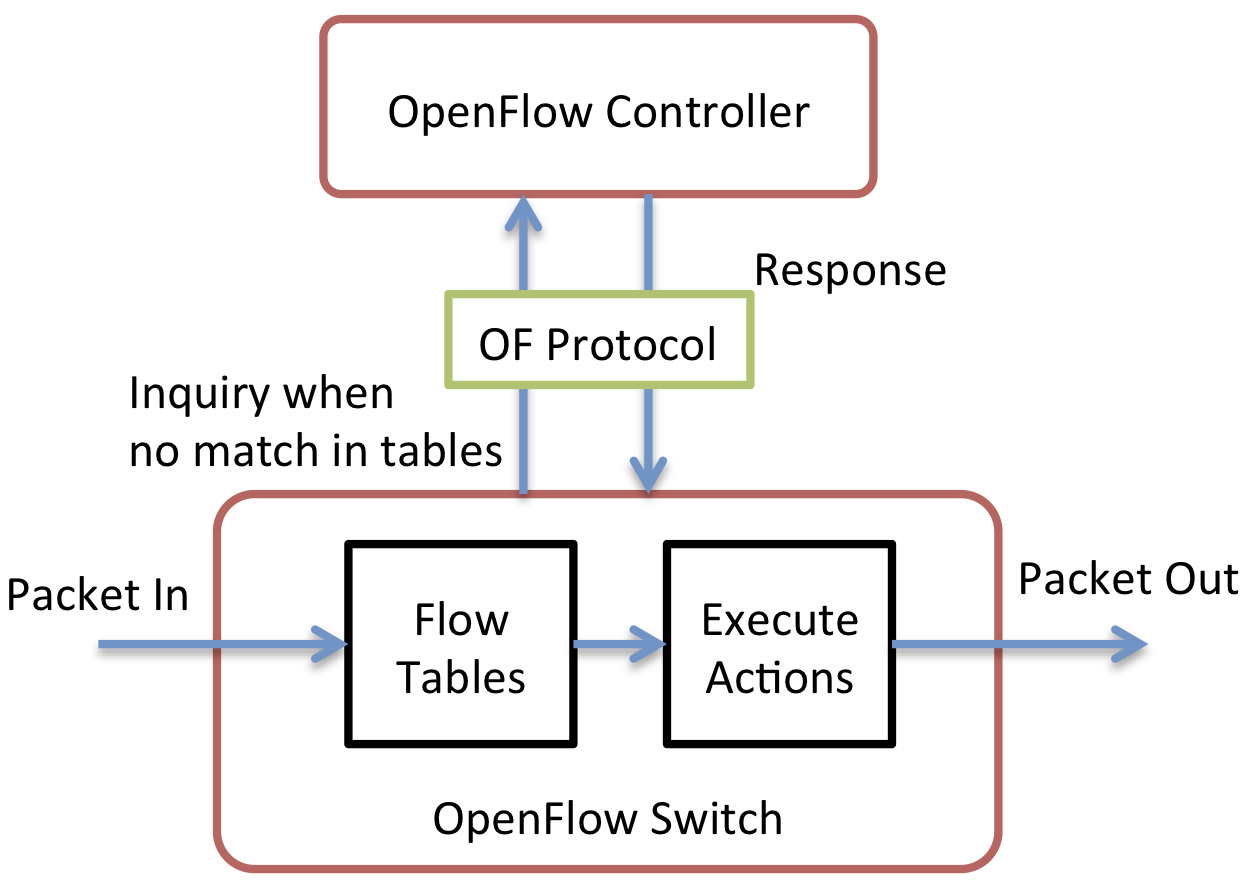
\includegraphics[width=0.95\linewidth]{openflow-paket-incoming}
	\caption{Eingehendes Paket bei OpenFlow}
	\label{fig:openflow-paket-incoming}
\end{figure}
		\subsection{Controller}
Das größte Bedenken bei ausgelagerten Controllern ist, dass die Performance und Skalierbarkeit darunter leidet. Aktuelle Tests mit den OpenFlow Controllern zeigen, dass diese durchaus bei großen Netzwerken mit mindestens 50000 neuen Flow-Requests pro Sekunde zurechtkommen \cite{nox-mt}. Es gibt bereits hoch-skalierbare Controller (NOX-MT) die acht Kerne nutzen und so 1,6 Millionen Flow-Requests pro Sekunde bei sehr geringer Latenz verarbeiten können. Es können weiterhin mehrere Controller genutzt werden, um zum einen die Performance, als auch die Ausfallsicherheit, was bei einem zentralen System von großer Bedeutung ist, zu verbessern. Es gibt auch dezentralisierte Controller, wie zum Beispiel Onix (closed source) und HyperFlow \cite{hyperflow}, dort werden logisch zentrale Controller aus physikalisch dezentralen Controllern erstellt. Ebenfalls gibt es Hybridlösungen, bei denen zum einen lokale Controller für lokale Entscheidungen, als auch globale zentrale Controller für weiterreichende Entscheidungen kontaktiert werden.
		\subsection{Southbound-API}
Die Kommunikation zwischen Gerät und Controller wird auch als „Southbound Communication“ bezeichnet. In OpenFlow erfolgt diese mit \gls{tls} verschlüsselt.
		\subsection{Northbound-API}
Die Kommunikation von Controller mit externen Anwendungen  wird auch als „Northbound Communication“ bezeichnet. Die Schnittstelle wird ebenfalls für Controller-Controller Kommunikation genutzt.
		\subsection{Standardarisierung}
		\begin{itemize}
			\item Die \gls{ietf} hat an Standardisierungen für ForCES im Bezug zu Protokollen sowie Mechanismen und Schnittstellen gearbeitet.
			\item Die \gls{onf} hat an der Standardarisierung von OpenFlow gearbeitet.
		\end{itemize}



\section{SDN Anwendungen}
	\subsection{Enterprise Netzwerke}
	Große Unternehmen haben sehr große Netzwerke die ein hohes Maß an Sicherheit verlangen. SDN können genutzt werden um Firewalls, Loadbalancer, \gls{nat}'s sowie Netzwerk \gls{acl}'s zu ersetzen. Durch diese Umstellung fallen fast alle sogenannten „Middleboxes“ weg, was zu einer deutlichen Vereinfachung der Konfiguration sowie des Verwaltungsaufwandes führt.
	\subsection{Rechenzentren}
	Die Netzwerke in Rechenzentren sind oft überdimensioniert um einem hohen Peak an Anforderungen standzuhalten. Daraus resultiert, dass diese im Allgemeinen nicht alle Ressourcen ausnutzen. In solchen großen Rechenzentren spielt der Aspekt des Stromverbrauchs eine große Rolle, hier kann \gls{sdn} helfen die Kosten zu reduzieren. Durch das Finden eines optimalen Netzwerkteils der für den aktuellen Bedarf ausreicht und das Ausschalten der nicht benötigten Geräte wird bis zu 60\% an Energie gespart. Allerdings hat SDN auch Performanceeinbußen bei reinen high-performance Netzwerken \cite{6730793}, was durch das Ständige auslagern von Anfragen an den Controller zustande kommt. Im Gegenzug wurden weitere Frameworks vorgestellt, die einem solchen Verhalten, durch die Verlagerung der meisten Flows zurück in den Switch, entgegenwirken. Ein praktisches Beispiel für den Einsatz von OpenFlow verbundenen Rechenzentren wurde 2012 von Google beim Open Network Summit vorgestellt, hierbei liefen viele Links bei annährend 100\% Auslastung.
	\subsection{Heim- und Kleinbetriebe}
	Gerade durch die niedrigen Kosten von Netzwerkgeräten haben viele kleine Firmen bereits ein relativ komplexes Netzwerk. Um nicht durch Malware verseucht zu werden spielt auch die Sicherheit eine große Rolle und eine Änderung der Konfiguration des Netzes sollte keine Ausfälle verursachen. Oft ist es auch nicht möglich in jedem Büro einen Netzwerkadministrator zu haben. Hier könnte ein \gls{sdn}, durch remote verwalteten Switche und Verteiltes Monitoring zur Erkennung von Sicherheitsproblemen, helfen.

\section{Zukunft \& Zusammenfassung}
\begin{itemize}
	\item Controller und Switch
	SDN haben Skalierungs-, Performance- und Sicherheitsherausforderungen \cite{6739370}, welche bereits durch Forschungsarbeiten aufgearbeitet und minimiert werden. Physikalisch dezentrale aber logisch zentrale Controller erweisen sich als wesentlich robuster und besser skalierbar als ein zentraler Controller, Beispiele solcher Controller sind Onix, Kando und HyperFlow.
	\item Das Internet mit SDN
	Die Natur eines zentralen Controllers widerspricht der dezentralen Struktur des Internets, allerdings ist eine logisch zentrale, aber physikalisch dezentrale Struktur der beteiligten \gls{as} denkbar. Es gibt bereits ein paar Versuche dieser Idee die auf \gls{mpls} basieren und Aufgaben an Geräte innerhalb des Bereichs oder außerhalb des Bereichs weitergeben. Ein weiterer Ansatz nutzt NOX und OpenFlow  um \gls{bgp}-ähnliche Funktionalität für das Routing innerhalb eines AS nutzbar zu machen.
	\item Virtualisierung
	Clouddienstleister und Virtualisierungsanbieter haben hohe Anforderungen an ihre Netzwerkinfrastruktur, schließlich müssen neue Virtuelle Maschinen (VM) oder Container innerhalb kürzester Zeit bereitgestellt werden. Ebenfalls muss ein hoch skalierbares Netzwerk-backend vorhanden sein, dass sich dynamisch den Anforderungen anpasst. Hierfür gibt es bereits Lösungen wie zum Bespiel Floodlight welches in OpenStack genutzt werden kann, oder NOX für MirageOS. LIME \cite{lime}, ein Design zum effizienten migrieren von Virtuellen Maschinen wurde ebenfalls vorgestellt.
\end{itemize}
\newpage
\section{Glossar}
	\listoffigures
	
	%Glossar
	\printglossary[style=altlist,title=Glossar]
	
	%Literaturverzeichnis & Style
	\bibliographystyle{plainnat}			
	\bibliography{literature} 
	
\end{document}

